\documentclass[12pt]{article}
% Language setting
\usepackage[english]{babel}
\usepackage{graphics}
\usepackage[draft]{graphicx}
\usepackage{fancyhdr} 
\usepackage{placeins}

% Set page size and margins
% Replace `letterpaper' with `a4paper' for UK/EU standard size

\usepackage[a4paper,top=2.0cm,bottom=2.54cm,left=2.54cm,right=2.54cm,marginparwidth=1.75cm]{geometry}

\usepackage{tocloft}
\usepackage[utf8]{inputenc}
\usepackage[T1]{fontenc}
\usepackage{lmodern} %change the name in the brackets in order to change the 
\renewcommand*\familydefault{\sfdefault}  %% Only if the base font of the document is to be sans serif

% Useful packages
\usepackage{amsmath}
\usepackage{graphicx}
\usepackage[colorlinks=true, allcolors=blue]{hyperref}
\usepackage{float}
\usepackage{algorithm}
\usepackage{algpseudocode}
\usepackage{pifont}
%\renewcommand{\bibname}{References} %to change the reference title



%-------------------------BEGIN DOCUMENT----------------------------------%
\begin{document}
\begin{titlepage}
\title{Optimized Condensation for Energy Storage:
Thermodynamics and Modeling}
\author{Omry Magen}

\newcommand{\HRule}{\rule{\linewidth}{0.5mm}} % Defines a new command for the horizontal lines, change thickness here

%----------------------------------------------------------------------------------------
%	LOGO SECTION
%----------------------------------------------------------------------------------------

% 
\includegraphics[width=8cm]{Figures/Logo.png}\\[1cm] 
 
%----------------------------------------------------------------------------------------

\center % Center everything on the page

%----------------------------------------------------------------------------------------
%	HEADING SECTIONS
%----------------------------------------------------------------------------------------

\vspace*{3cm}
\textsc{\Large Imperial College London}\\[1.5cm] % Major heading such as course name
\textsc{\large Department of Mechanical Engineering}\\[0.5cm] % Minor heading such as course title
\textsc{\large Advanced Mechanical Engineering Course}\\[1.5cm] % Name of your university/college

%----------------------------------------------------------------------------------------
%	TITLE SECTION
%----------------------------------------------------------------------------------------
\makeatletter

{ \huge \bfseries \@title}\\[1cm] % Title of your document

 
%----------------------------------------------------------------------------------------
%	AUTHOR SECTION
%----------------------------------------------------------------------------------------




\begin{minipage}{0.4\textwidth}
\centering \large
By:\\
\@author % Your name            
\end{minipage}\\[0.1cm]


\begin{minipage}{0.4\textwidth}
\centering \large
BSc. Mechanical Engineering at Technical University Berlin \\[1.2em] % Supervisor's Name           
\end{minipage}\\[1cm]
\makeatother % If you don't want a supervisor, uncomment the two lines below and remove the section above       
 % \Large\@author\\[3cm] % Your name                %----------------------------------------------------------------------------------------        %    DATE SECTION        %---------------------------------------------------------------------------------------- 
 \begin{minipage}{1\textwidth}
    \centering \large
    A thesis submitted in partial fulfillment of the requirements for the Master of Science Degree of  Imperial College London and the Diploma of Membership of Imperial College \\[0.9cm] 
    {\today}\\[0.1cm] 
    \begin{center}
        Word Limit: 18,000\\
        Word Count: 16,240     
    \end{center}
\end{minipage}\\ 
                  
 % Date, change the \today to a set date if you want to be precise 
% \vspace*{\fill}




\makeatother
 % Fill the rest of the page with whitespace

\end{titlepage} 
\newpage

\addcontentsline{toc}{section}{Abstract}
\pagenumbering{Roman}
\section*{Abstract}
A research project has been initiated to gain a deeper understanding of the condensation phenomenon, and potentially implement numerical models to capture the physics driving this process. This report focuses on the progress achieved, modifications that have been made since the start of the project and a discussion on future work. The achievements involve selecting appropriate conservation equations and nucleation models that will potentially allow the condensation phenomenon to be accurately simulated within a low-pressure steam turbine. Furthermore, a droplet growth model based on the $d^2$ evaporation model will be introduced. This model has been derived and implemented in a code that will be presented in the form of a Pseudocode. Results from a parametric analysis of this model will be displayed and accompanied by a brief discussion. 
\thispagestyle{empty}
\newpage
\hypersetup{linkcolor=black}
    \tableofcontents

\thispagestyle{empty}


\listoffigures

\newpage

\pagenumbering{arabic} 

\section{Introduction}
Simulating compressible multiphase flows continues to be a challenging technical problem due to the complex nature of the physics involved. Numerical methods have been developed in recent years to reduce the computational burden of such simulations and to enable them to have industrial use. The case of condensing flows is under investigation, as it is a phenomenon that is widely observed in different technical applications. Moreover, unwanted condensation which is found in a low-pressure steam turbine is of special interest, because mitigating this phenomenon can lead to higher turbomachinery efficiencies and thus to "greener" power generation \cite{francesco2017cfd}. However, when simulating multiphase flows, several assumptions must be made regarding the interaction between two phases as well as the nature of vapor nucleation and droplets growth given their existence. 

This report presents the current progress achieved on this topic to this date. At first, the project's milestones reached will be enumerated, followed by a thorough depiction of the findings made. These include condensation models that were found and presenting results of simulations that were carried out. Then, modifications to the original project plan will be presented with an updated Gantt diagram. Finally, the report's conclusions will be presented along with a discussion of forthcoming project work. 



\newpage
\section{Achievements}
The project milestones were consistently achieved within the project’s time frame. With reference to the project objectives, the corresponding achievements are listed as follows:\\\\
\noindent
\textbf{Objective 1}: Achieving a fundamental understanding of the physical and thermodynamical process known as condensation and deriving appropriate models:\\
$\rightarrow$Following a review of the literature, a better understanding of the topic has been achieved and appropriate models have been selected that are necessary to simulate a multiphase flow. These include:
\begin{enumerate}
        \item Conservation equations.
        \item Nucleation model.
        \item Droplet growth model.
\end{enumerate} 
\noindent
\textbf{Objective 2}: Implement an analytical approach to simulate the condensation of a suspended droplet:\\
$\rightarrow$A droplet growth model for a single suspended droplet has been implemented in Python.\\\\
\textbf{Objective 3}: Execute a parametric analysis, testing boundary conditions:\\
$\rightarrow$A parametric analysis has been performed to gain a deeper understanding of the droplet growth model limitations and assess the integrity of the simulated physics.\\\\
\noindent
These achievements are briefly discussed in the following subsections. Moreover, project objectives that remain or that have been modified will be discussed in Section \ref{s:modifications}.
\subsection{Conservation Equations and Nucleation Model}\label{s:model}
Recent literature concerning simulating a multiphase flow within a low-pressure steam turbine suggests that the Eulerian/ Eulerian frame of reference is favored over other methods due to substantially lower computational costs involved with such simulations; This method utilizes volume averaging of the liquid phase equations, which results in lower accuracy compared to the direct tracking of droplet trajectories of the Eulerian/Lagrangian approach \cite{francesco2017cfd}. This suggests that if the accuracy of these simulations can reach satisfactory levels, they may have technical applications, for example, in the industry. For these reasons, this approach was chosen as the formulation of the conservation equations. Firstly, the conservation of mass for the vapor, liquid and the conservation of the droplet number are formulated respectively \cite{patel2016influence}:
\begin{equation}
    \frac{\partial}{\partial t}(\rho_{v}\alpha_{v})+\frac{\partial}{\partial x_{j}}(\rho_{v}\alpha_{v}u_{j,v}) = -\sum S_{d}-\sum m^{*}\alpha_{v}J_{d}  
    \label{eq:v_conti}
\end{equation}
\begin{equation}
    \frac{\partial}{\partial t}(\rho_{l}\alpha_{l})+\frac{\partial}{\partial x_{j}}(\rho_{l}\alpha_{l}u_{j,l}) = \sum S_{d}+\sum m^{*}\alpha_{v}J_{d}  
    \label{eq:l_conti}
\end{equation}
\begin{equation}
     \frac{\partial}{\partial t}(\rho_{l}\eta)+\frac{\partial}{\partial x_{}}(\rho_{l}\eta u_{j,l}) = \rho_{l}\alpha_{v}J_{d}  
    \label{eq:number_conti}
\end{equation}
The drag effect between the phases caused by the droplets is considered negligible because 90\% of the droplet’s mass concentration consists of sub-micron droplet sizes. Thus, the velocities of the two phases are assumed to be identical \cite{patel2016influence}. The conservation of momentum is therefore only formulated for the vapor phase based on the well-known Reynolds-averaged Navier-Stokes (RANS) formulation:
\begin{equation}
    \frac{\partial}{\partial t}(\rho_{v}\alpha_{v}u_{i,v})+\frac{\partial}{\partial x_{j}}(\rho_{v}\alpha_{v}u_{i,v}u_{j,v}) = -\alpha_{v}\frac{\partial P}{\partial x_{i}}+\frac{\partial}{\partial x_{j}}(\alpha_{v}\tau_{ij,v}) + S_{F,m} 
    \label{eq:v_momentum}
\end{equation}
Finally, the conservation of energy is formulated:

\begin{equation}
    \frac{\partial}{\partial t}(\rho_{v}\alpha_{v}H_{v})+\frac{\partial}{\partial x_{j}}(\rho_{v}\alpha_{v}u_{i,v}H_{v}) =-\alpha_{v}\frac{\partial P}{\partial t}+\frac{\partial}{\partial x_{j}}(\alpha_{v}\Gamma _{E}\frac{\partial T_{v}}{\partial x_{j}})+\frac{\partial}{\partial x_{j}}(\alpha_{v}u_{i,v}\tau_{ij,v}) + S_{E} 
    \label{eq:v_energy}
\end{equation}
These equations follow the traditional nomenclature of the velocity components ($u_{i}$), temperature ($T$), pressure ($P$), density ($\rho$), phase volume fraction ($\alpha$) and thermal diffusion coefficient ($\Gamma_{E} $). In addition, the number of liquid droplets per unit volume ($\eta$), the mass of a stable nucleus ($m^*$) and the nucleation rate defined as the number of droplets generated per unit volume ($J_{d}$) are also introduced. Subscript $v$ and $l$  refer to the vapor phase and liquid phase respectively. Furthermore, the interaction between the two phases is facilitated through the mass ($S_{d}$), momentum ($S_{F,m}$) and energy ($S_{E}$) source terms. These will not be further discussed, however, a thorough description of these was presented by Gerber and Kermani \cite{gerber2004pressure}.

$J_{d}$ can be modeled in various ways, however, it was found in the review of the literature that nucleation i.e condensation under non-equilibrium and homogeneous conditions were the leading phenomenon found in a low-pressure steam turbine. Here, the term non-equilibrium is referred to the state in which the vapor is found when condensing; considering the case of an expansion in a low-pressure steam turbine, the vapor may not condense directly when entering the two-phase region but rather enter a state of supersaturation, where activation energy is then needed to trigger the phase change. Furthermore, it should be noted that homogeneous refers to nucleation which is not triggered by a cool surface to overcome this activation barrier. The aim was therefore to find a model which performs well under the aforementioned conditions, and thus the Diffuse Interface Theory proposed by Gránásy et. al \cite{granasy1993diffuse} will be implemented. For crucial parameters such as the droplet count (amount of formed droplets), this model's performance was in good agreement with the experimental findings \cite{granasy1993diffuse}, which will presumably increase the accuracy of such multi-phase simulations. The model is defined as follows:
\begin{equation}
    J_{d}=J_{0}\exp{\frac{-\Delta \Omega^*}{\kappa T}}
    \label{eq:nucleation}
\end{equation}  
where $\kappa$ is the Stefan Boltzmann constant and $J_{0}$ is a factor depending on the kinetics of an investigated system. The free energy barrier, $\Delta\Omega^*$, is defined as
\begin{equation}
    \Delta\Omega^*=-\frac{\frac{4\pi}{3}(R_{S}-R_{H})^{3}\Delta h_{0}T \Delta s_{0}}{\Delta h_{0}+T \Delta s_{0}-2\sqrt{\Delta h_{0}T \Delta s_{0}}} 
\label{eq:critical_drop}
\end{equation}
where $\Delta h_{0}$ and $\Delta s_{0}$ are the enthalpy and entropy of the droplet. Gránásy et. al defined the free energy barrier as the critical work of droplet formation which assumes that the droplet is characterized by the properties of the bulk. The diffuse interface between the phases is assumed and is independent of the droplet size. Thus, the difference between $R_{S}$ and $R_{H}$ i.e the position of the entropy and enthalpy surfaces is constant and dependent only on the level of supersaturation. Figure \ref{f:granasy} presents a schematic illustration of these surfaces. 

\begin{figure}[H]
    \centering
    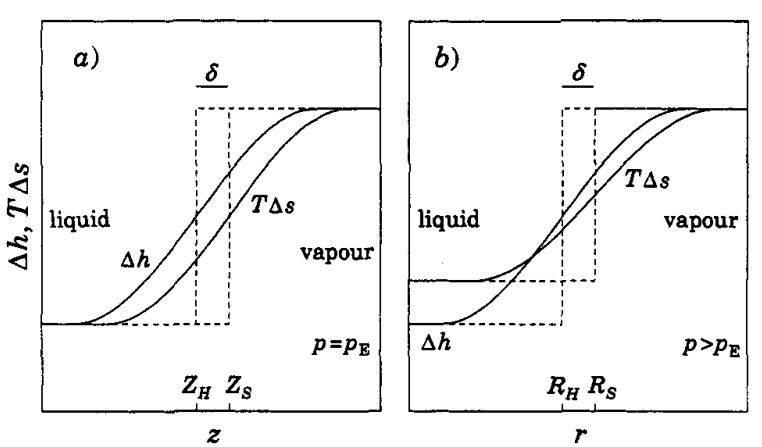
\includegraphics[width=0.6\textwidth]{Figures/Granasy_plot.png}
    \caption{Cross-interfacial enthalpy and entropy concept for a) planar interface geometry in equilibrium and b) curved interface geometry for supersaturated conditions \cite{granasy1993diffuse}}
    \label{f:granasy}
\end{figure}
This nucleation model along with the conservation equations will require the use of water thermodynamic properties which will be integrated into CFD simulations. Further details will be discussed in Section \ref{s:future_work}.
\subsection{Droplet Growth}\label{s:droplet}
The well-known $d^2$ evaporation model depicts the evaporation phenomenon of a single suspended droplet within an infinite space under steady and equilibrium conditions \cite{turns2011introduction}. It was found that by adjusting the boundary conditions and tuning certain parameters, the reversed process can be described i.e condensation. 
The derivation of the droplet growth rate is centered around the conservation of species and energy which are integrated across the interface of the droplet itself. In radial coordinates, the species is given by
\begin{equation}
    r^{2}\rho u \frac{\partial Y}{\partial r}-\frac{\partial}{\partial r}\left(r^{2} \rho D \frac{\partial Y}{\partial r}\right) =0
\end{equation}
and energy by
\begin{equation}
    r^{2}\rho u \frac{\partial c_{p}T}{\partial r}-\frac{\partial}{\partial r}\left(\frac{\lambda}{c_{p}}r^{2} \rho  \frac{\partial c_{p}T}{\partial r}\right) =0
\end{equation}
where $D$, $\lambda$ and $c_{p}$ are the molecular diffusivity of water in the air, thermal diffusivity and specific heat capacity respectively. 
By utilizing the conservation of mass for the two phases, one can acquire the following relationship between the mass flow and thermal heat rate
\begin{equation}
    \dot{m}=-2\pi\rho_{v}D\cdot r \cdot Sh\cdot \log(1+B_{m})
\end{equation}
\begin{equation}
    q=-\dot{m}\cdot \frac{c_{p}(T_{inf}-T_{s})}{B_{t}}-h_{lat}
\end{equation}
where $Sh$ is the Sherwood number, $B_{m}$ and $B_{t}$ the Spalding mass and heat transfer numbers respectively (defined in Algorithm \ref{alg:droplet}), $T_{inf}$ the temperature of the surrounding air and $T_{s}$ the temperature at the droplet surface, which is assumed to be uniform throughout the droplet. $h_{lat}$ is the latent heat of condensation. Using these derived equations, an algorithm based on the work of Abramzon and Sirignano \cite{abramzon1989droplet} was implemented in Python to simulate the physics of the droplet growth. How the algorithm operates is conceptualized in Algorithm \ref{alg:droplet}. 

\begin{algorithm}
    \caption{Simplified droplet growth concept}
    \label{alg:droplet}
    \begin{algorithmic}[1]
    \State \textbf{Initialize}: Boundary Conditions: $T_{s}$, $T_{inf}$, $P_{amb}$, $r_{0}$ \Comment{$r_{0}$: initial droplet size}
    \State \textbf{Initialize}: $dt$, $q_{out}$ \Comment{time step and manual thermal energy extraction}
    \State \textbf{Compute}: $P_{sat,inf}$ at $T_{inf}$\\ 
    \quad \quad \quad \quad \quad $P_{sat,s}$ at $T_{s}$ \\
    \quad \quad \quad \quad \quad$Y_{inf}$ from $P_{sat,inf}$ \& $P_{amb}$ \\
    \quad \quad \quad \quad \quad$Y_{s}$ from $P_{sat,s}$ \& $P_{amb}$\\
    \quad \quad \quad \quad \quad$m$ from $r_{0}$ \& $\rho_{l}$ \Comment{$m$: initial mass of droplet}
    \For{\emph{total number of iterations} }
    \State \textbf{Compute}: $\rho_{g}$, $c_{p}$, $\kappa_{g}$, $\mu_{g}$, $D$ \Comment{Using one third law averaging at $T_{s}$ \& $T_{inf}$}
    \State \textbf{Compute}: $Sh$, $Nu$ \Comment{Sherwood and Nusselt numbers}
    \State $B_{m}=(Y_{s}-Y_{inf})/(1-Y_{s})$
    \State $\dot{m}=-2\pi\rho_{v}D\cdot r \cdot Sh\cdot \log(1+B_{m})$
    \State $B_{t}=c_{p}(T_{inf}-T_{s})/h_{lat}$ \Comment{Value is iteratively corrected using $Sh\: \&\: Nu$}
    \State $q=-\dot{m}\cdot (c_{p}(T_{inf}-T_{s})/B_{t})-h_{lat}$
    \State $r_{s}=\sqrt[3]{(3/4\pi \rho_{l})\cdot m+\dot{m}\cdot dt}$
    \State $m=r_{s}^{3}\cdot \rho_{l}\cdot 4\pi/3$
    \State $T_{s}=(6 dt(q-q_{out}))/(c_{p}(m+\dot{m}\cdot dt))+T_{s}$
    \State \textbf{Recompute}: $P_{sat,s}$ at $T_{s}$
    \State \textbf{Recompute}: $Y_{s}$ from $P_{sat,s}$ \& $P_{amb}$
    \EndFor
    
    \end{algorithmic}
\end{algorithm}

 At this point, it is necessary to mention that the pressure at the droplet surface was calculated under the assumption of saturation conditions. In this context, it is clear that there is a degree of contradiction between the assumption of non-equilibrium conditions in the flow and the equilibrium conditions at the droplet surface. Thus, it is expected that an adjustment of the code might be necessary. Section \ref{s:future_work} will provide further elaboration on this topic. Furthermore, $q_{out}$ is an additional source term introduced to the algorithm to simulate artificial thermal energy extraction out of the droplet to assess its influence on droplet growth. Extracting heat can not only provide an additional understanding of the model's physics integrity but also serve as a basis for intuition when testing future cases under different field conditions.

A parametric analysis of the boundary conditions was performed to assess the limitations of the model and the feasibility of acquiring physical results. The ambient pressure varied between $1$ and $2$ bars, while the temperature difference between the droplet and the air $dT$ varied between $10$ and $20$ K. Here, $T_{s}$ was held constant at $350$ K. Within these case studies, $q_{out}$ was also iterated for values that are consistent with the order of magnitude of the cases under inspection. This results in a total of $16$ different test cases which are presented. It should also be mentioned, that the initial droplet radius ($r_{0}$) was equal to $1e-6$ m. This value is considered as a typical newly condensed droplet size in a low-pressure steam turbine \cite{patel2016influence}.  In Figure \ref{f:T_s}, the evolution of the droplet temperature with time was plotted for all aforementioned cases. Firstly, considering Figure \ref{f:T_s} (a) and (b), where the pressure is equal to $1$ bar, the balance between the thermal energy transferred into the droplet due to temperature difference and the energy being extracted from the droplet artificially can be well observed; for little extraction, the temperature would rise quickly until convergence. The value to which the temperature will initially converge is presumably dictated by the point where the temperature difference (surrounding air heating the droplet) is at balance with the artificial extraction.

\begin{figure}[H]
    \centering
    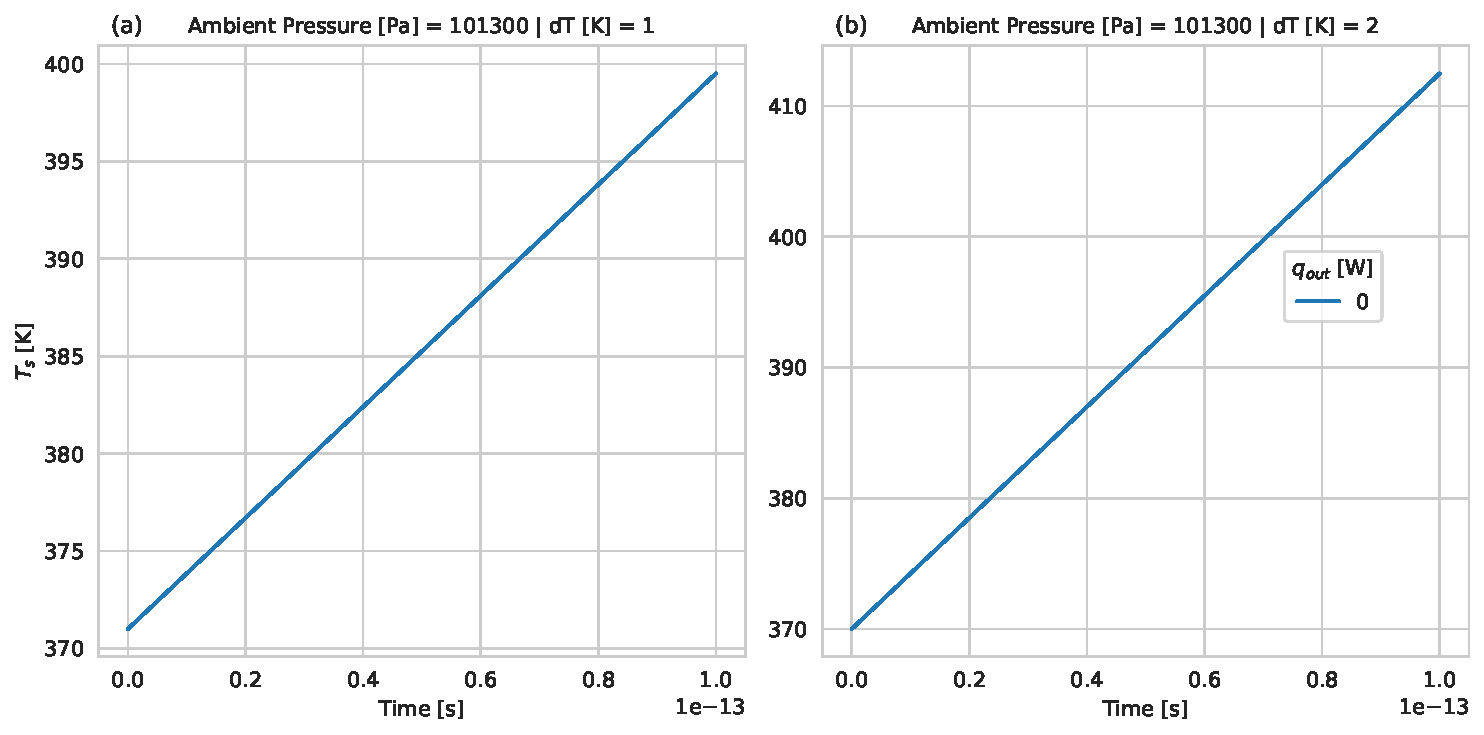
\includegraphics[width=1\textwidth]{Figures/T_s.pdf}
    \caption{Doplet surface temperature as a function of time for four different boundary conditions}
    \label{f:T_s}
\end{figure}

Nevertheless, when increasing the heat extraction, the temperature would initially converge, but then start to increase again and the rate at which it increases is dependent on the rate of extraction. Similar behavior can be well observed for the pressure of $2$ bars (Figure \ref{f:T_s} (c) and (d)) but the higher pressure increases the initial convergence temperature. This could be possibly explained by the steady mass increase of the droplet.

For these test cases, the evolution of the droplet radius with time is illustrated in Figure \ref{f:r_s}. It can be directly observed that for all boundary conditions, the rate at which thermal heat is extracted is directly correlated to the droplet's growth rate. This was anticipated and demonstrates physical properties, as evident from the preceding diagram, that a greater heat extraction causes the droplet to cool down, which suggests that since the mass flow rate is correlated to thermal heat transfer, the droplet will enlarge more rapidly. Interestingly, the radius of the droplet will initially have a different growth rate depending on the boundary conditions, until it reaches its steady growing state. The "initial transient period" was also identified by Turns \cite{turns2011introduction} in the experimental data presented for the evaporation case, where the same behavior was observed. In the case of evaporation, this is correlated to the time it takes the droplet to reach boiling temperature. Here, it is presumably associated with the droplet reaching a steady state temperature difference which is sufficient for steady droplet growth. 

\begin{figure}[H]
    \centering
    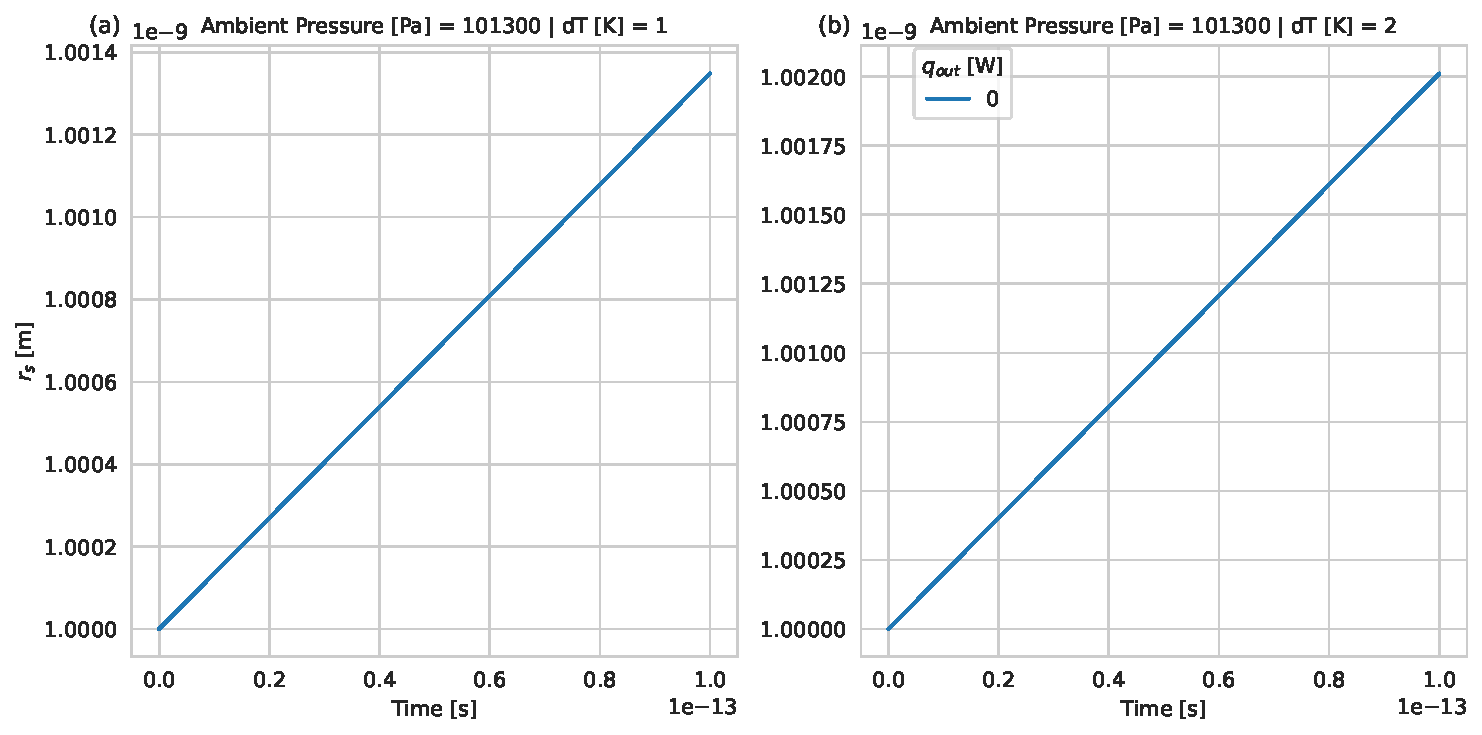
\includegraphics[width=1\textwidth]{Figures/r_s.pdf}
    \caption{Doplet radius as a function of time for four different boundary conditions}
    \label{f:r_s}
\end{figure}
In the Appendix, the squared time derivative of the droplet's radius is also presented. In reference to Figure \ref{f:r_s}, it was shown that for the different field conditions, the initial transient period is well observed and quickly after, the radius will enter a state of constant growth rate. It should be noted, that in the special case of $q_{out}=0$, the droplet will reach ambient temperature and will stop growing.
\newpage
\section{Project Modifications}\label{s:modifications}
A few noticeable modifications have been made to the project Gantt diagram since the beginning of the project. Following the literature review, the project focus shifted to the condensation phenomenon in a more technical context. Thus, it will focus on assessing the condensation phenomenon inside a low-pressure steam turbine. The objectives are therefore newly stated, omitting the objectives that have been accomplished up to this point:
\begin{itemize}
    \item Implement the Eulerian-Eulerian approach into OpenFOAM.
    \item Implement the Diffuse Interface nucleation model into OpenFOAM.
    \item Implement the reversed $d^{2}$ law as a droplet growth model into OpenFOAM.
\end{itemize}
The modified Gantt diagram is presented in Figure \ref{f:Gannt}. It should be noted that the above-mentioned objectives are abbreviated in the form of the project's milestones $D$ and $E$.

\noindent
The main modifications made to the Gantt diagram are listed as follows:
\begin{itemize}
    \item No film or surface condensation models will be explored.
    \item Species analysis will only be performed in the case of sufficient progress within the project's time frame.
    \item Other numerical approaches such as Eulerial-Lagrangian frame of reference will only be explored in the case of sufficient progress within the project's time frame.
\end{itemize} 
It can be seen that time allocation to different aspects of the project has been redistributed due to the project's modifications. Noticeably, more time has been allocated to the modification of the OpenFOAM solver, as it has introduced some technical difficulties up to this point. Furthermore, milestones have been readjusted to fit the new project objectives. 
\begin{figure}[H]
    \centering
    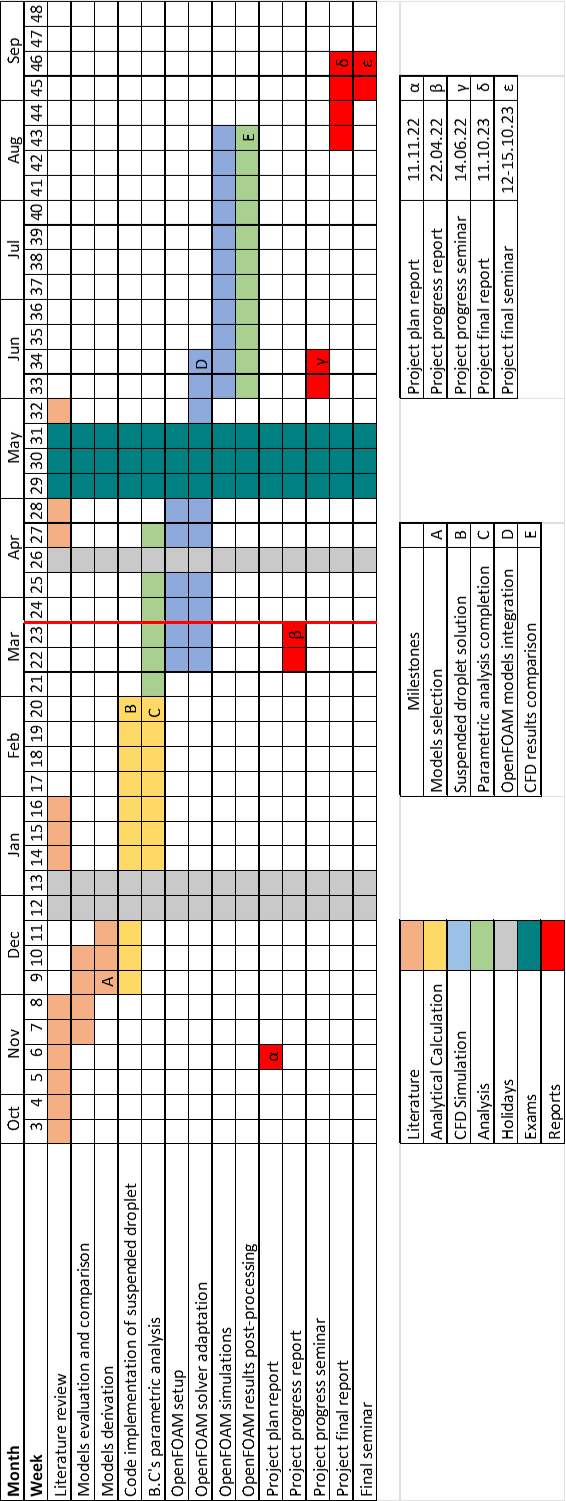
\includegraphics[width=0.52\textwidth]{Figures/Gantt.png}
    \caption{Updated Gannt diagram}
    \label{f:Gannt}
\end{figure}
\newpage
\section{Future Work}\label{s:future_work}
Future work includes the newly formulated objectives from Section \ref{s:modifications}. Two foreseen technical challenges are expected in the first steps toward achieving these objectives:
\begin{enumerate}
    \item To ensure that the solver has access to both liquid and vapor properties under different field conditions, it is necessary to implement water properties tables within OpenFOAM. This is particularly important in steam turbines where the field conditions can vary widely.
    \item The assumptions of non-equilibrium nucleation will presumably require an adaptation of the $d^2$ growth model, due to the assumed saturation conditions at the droplet surface. Nevertheless, literature exists that will support such modifications.
\end{enumerate}
The implementation of the Eulerian-Eulerian approach and the Diffuse Interface theory will require learning basic skills in the languages $C$ and $C++$, the used programming language in OpenFOAM. The software is based on the principles of Object-Oriented Programming, therefore, any difficulties that arise are likely to be related to the language itself rather than how the program operates. 

To ensure that the targeted simulations are accurate, the appropriate meshing of a turbine cascade is required. Comparisons between experimental and computational results seen in the literature suggest that assuming a 2D flow (one cell depth) with periodic boundary conditions above the suction side and below the pressure side of the blade can often be sufficient to capture flows in a turbine cascade. This reduces further the computational burden of such simulations and the meshing itself will remain relatively simple. The conclusion was that this aspect of the project would not pose any extraordinary difficulties and therefore it was not included in the Gantt diagram.
\newpage
\section{Conclusions}
The report explored the progress of the project with the main goal of modeling the physics of the multiphase condensing flows. The objectives of the project have been slightly modified since the project start to simulate the condensation phenomenon inside a low-pressure steam turbine. These modifications have been presented in a Gantt diagram. In the context of steam turbines, a literature review has been performed and conservation equations and a nucleation model has been chosen; the Eulerian-Eulerian frame of reference will be utilized and the Diffuse Interface nucleation theory will be implemented to capture the physics of the condensation. Furthermore, a droplet growth model based on the well-known $d^2$ evaporation model has been implemented in a code. Given the droplet's existence, simulations were performed to capture the interaction of a suspended droplet with the surrounding air. A Pseudocode format was used to illustrate how to program operates. Lastly, executing a parametric analysis proved that the model yields physical results and these were briefly discussed. 

For future work, it was concluded that several technical aspects of the project will need to be overcome to reach the remaining project objectives. These include implementing water properties tables in OpenFOAM, familiarizing oneself with $C/C++$ programming for smooth implementation of the selected models and creating a 2D mesh for the turbine cascade. As a result, it was determined that the proposed project's timeline is adequate for achieving the project's objectives.






\cleardoublepage
\phantomsection
\addcontentsline{toc}{section}{References}

\bibliographystyle{ieeetr}
\bibliography{References}
\newpage
\appendix
\addcontentsline{toc}{section}{Appendix}
\section*{Appendix}\label{s:appendix}
\begin{figure}[H]
    \centering
    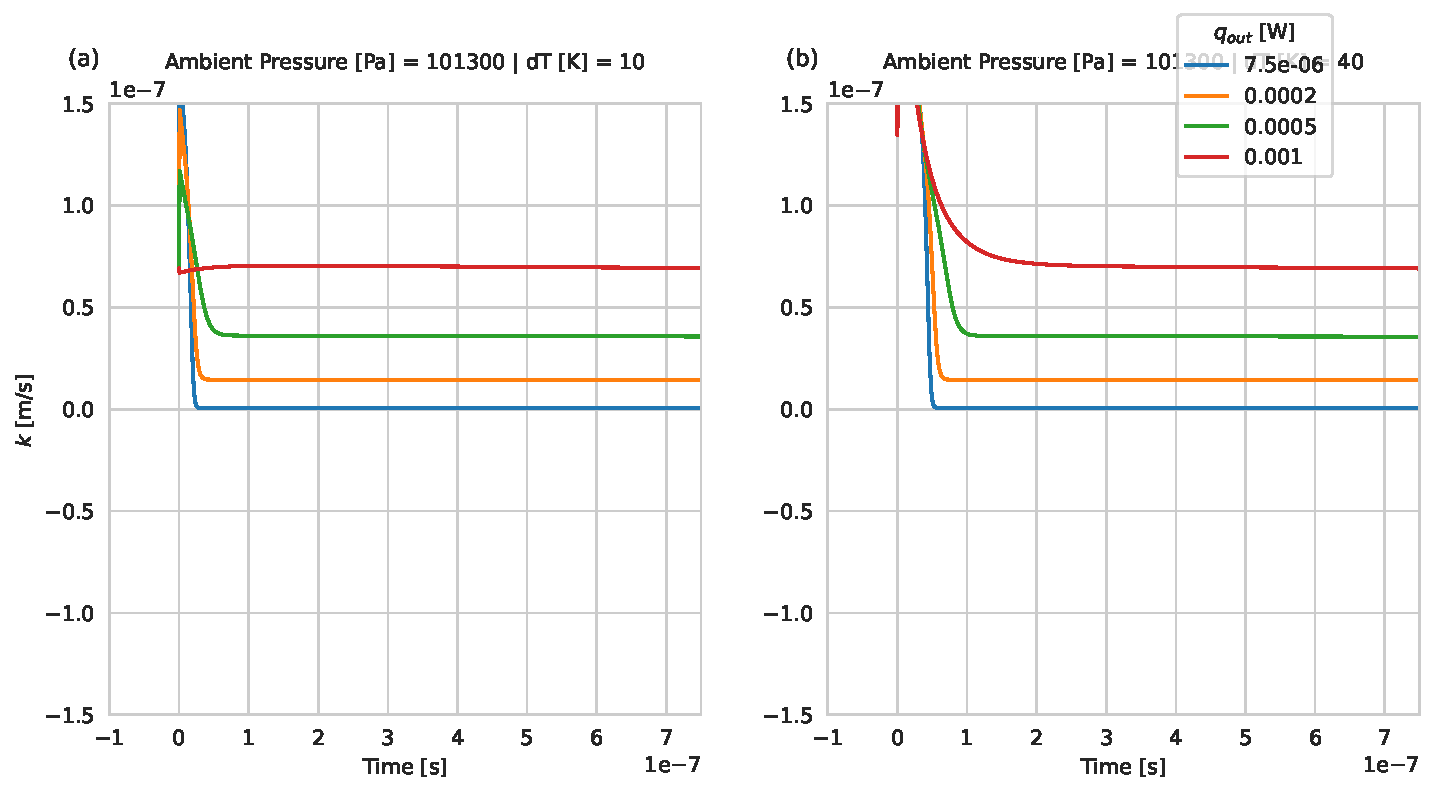
\includegraphics[width=0.9\textwidth]{Figures/k.pdf}
    \caption{Doplet squared growth rate as a function of time for four different boundary conditions}
    \label{f:k}
\end{figure}
\pagebreak
\end{document}